% Copyright 2026 Sreeram Anil
% SPDX-License-Identifier: CC-BY-4.0
\chapter{Marginalised (Rao--Blackwellised) particle filter (RBPF)}
\label{ch:rbpf}

\section*{At a glance}
\begin{tabular}{@{}l>{\raggedright\arraybackslash}p{0.76\textwidth}@{}}
Family & Sequential Monte Carlo (particle / ensemble / Gaussian sum) \\
Header & \texttt{include/estkit/particle/rbpf.hpp} \\
Model adapter & \texttt{include/estkit/battery/ecm\_mixed\_model.hpp} \\
Registered name & \texttt{RBPF} ($N=200$ particles, $n_n=2$ sampled states) \\
State dimension & $n_x = n_n + n_l = 2 + 2$ (cell model) — generic in $n_n, n_l, n_u, n_y$ \\
Cost per step & \SI{39.9}{\micro\second}/step ($84\times$ EKF); $\mathcal{O}(N(n_l^3 + c_f + c_h))$, no heap \\
Memory & \SI{34.0}{\kilo\byte} ($N$ particles, each with a $n_l$-mean and an $n_l\times n_l$ covariance) \\
Primary references & \cite{schon2005marginalized,doucet2000rbpf,chenliu2000mkf,casella1996rao} \\
\end{tabular}

\section{Motivation and aerospace/BMS relevance}
A particle filter pays for every dimension it samples.  The number of particles needed to cover a
posterior to a given accuracy grows exponentially with the dimension of the space being explored,
so the single most effective way to make sequential Monte Carlo affordable is to \emph{stop
sampling the states that do not need it}.

The 2-RC equivalent-circuit cell model is an unusually clean example of a model where most states
do not need it.  Of its four states, exactly two are responsible for all the nonlinearity: the
state of charge $\soc$, which enters the measurement through the curved $\ocv(\soc)$ map, and the
hysteresis level $h$, whose transition coefficient depends on the magnitude of the current.  The
other two --- the RC branch voltages $v_1$ and $v_2$ --- obey a \emph{linear} recursion with
coefficients that depend only on the (known) input, and they enter the measurement \emph{linearly}.
Conditioned on a trajectory of $(\soc, h)$, the pair $(v_1,v_2)$ is an exactly linear-Gaussian
system, so its posterior is available in closed form from a two-state Kalman filter.  Sampling it
is not merely wasteful, it is provably harmful: the Rao--Blackwell theorem says that replacing a
Monte-Carlo average by a conditional expectation can never increase the variance.

This is the marginalised particle filter of Schön, Gustafsson and Nordlund
\cite{schon2005marginalized} (equivalently the Rao--Blackwellised particle filter of Doucet, de
Freitas, Murphy and Russell \cite{doucet2000rbpf} and the mixture Kalman filter of Chen and Liu
\cite{chenliu2000mkf}).  It is the workhorse of aerospace terrain-aided and map-aided navigation,
where position is nonlinear in the map but velocity, attitude and sensor biases are conditionally
linear; Schön et al.\ report that the same partitioning reduces an aircraft navigation problem from
nine sampled dimensions to two.  For a battery it halves the sampled dimension and, as the
benchmark shows, buys a factor of three in nominal accuracy over a bootstrap filter with two and a
half times as many particles, at half the cost --- and the largest margin over the EKF of any method
in this family on the current-bias scenario.

\section{Problem statement and assumptions}
The RBPF requires a \emph{conditionally linear} ("mixed linear/nonlinear") model.  Partition the
state as $\vx = [\vx_n^\T\ \vx_l^\T]^\T$ with $\vx_n\in\real^{n_n}$ \emph{nonlinear} and
$\vx_l\in\real^{n_l}$ \emph{linear}, and assume
\begin{align}
  \vx_n(k+1) &= f_n\big(\vx_n(k),\vu(k)\big) + \vw_n(k),
    & \vw_n &\sim \N{\bm 0}{\mQ_n(\vx_n,\vu)}, \label{eq:rb-fn}\\
  \vx_l(k+1) &= \mA_l(\vu(k))\,\vx_l(k) + \bm{b}_l(\vu(k)) + \vw_l(k),
    & \vw_l &\sim \N{\bm 0}{\mQ_l(\vu)}, \label{eq:rb-fl}\\
  \vy(k) &= h_n\big(\vx_n(k),\vu(k)\big) + \mC_l\big(\vx_n(k),\vu(k)\big)\,\vx_l(k) + \vv(k),
    & \vv &\sim \N{\bm 0}{\mR(\vu)}. \label{eq:rb-h}
\end{align}
Two structural conditions do the work:
\begin{enumerate}[label=(C\arabic*),leftmargin=3em]
  \item \textbf{$f_n$ does not depend on $\vx_l$}.  The nonlinear states evolve autonomously given
        the input, so a sampled trajectory $\vx_n(0{:}k)$ can be generated without knowing $\vx_l$.
  \item \textbf{$\vy$ is affine in $\vx_l$}, with a coefficient matrix $\mC_l$ that may depend on
        $\vx_n$ and $\vu$ but not on $\vx_l$.
\end{enumerate}
Under (C1)--(C2), conditioned on $\vx_n(0{:}k)$ the remaining system \eqref{eq:rb-fl},
\eqref{eq:rb-h} is linear with Gaussian noise and \emph{known} (trajectory-dependent) coefficients,
so its posterior is exactly Gaussian.  Schön et al.\ also treat the general case in which
$\vx_n(k+1)$ contains a term $\mA_n\vx_l(k)$ and in which $\vw_n,\vw_l$ are correlated; both add
extra Kalman updates.  Neither occurs here (see Section~\ref{sec:rb-battery}), and the header
documents the omission.

\section{Derivation}

\subsection{The factorisation}
Bayes' rule applied to the joint trajectory posterior gives, with no approximation,
\begin{equation}
  p\big(\vx_n(0{:}k),\, \vx_l(k) \,\big|\, \vy(1{:}k)\big)
  \;=\;
  \underbrace{p\big(\vx_l(k)\,\big|\,\vx_n(0{:}k),\vy(1{:}k)\big)}_{\text{exactly Gaussian (Kalman)}}
  \;\cdot\;
  \underbrace{p\big(\vx_n(0{:}k)\,\big|\,\vy(1{:}k)\big)}_{\text{approximated by particles}},
  \label{eq:rb-factor}
\end{equation}
\cite[eq.~(6)]{schon2005marginalized}.  The RBPF represents only the second factor by samples,
\begin{equation}
  \hat p\big(\vx_n(0{:}k)\mid\vy(1{:}k)\big) = \sum_{i=1}^{N} w^i\,\delta\big(\vx_n(0{:}k) - \vx_n^i(0{:}k)\big),
  \label{eq:rb-particles}
\end{equation}
and attaches to particle $i$ the sufficient statistics $(\bar{\vx}_l^i, \mP_l^i)$ of the first
factor.  Each particle is therefore a \emph{point} in $\real^{n_n}$ carrying a \emph{Gaussian} in
$\real^{n_l}$, and the filtering density of the full state is the Gaussian mixture
\begin{equation}
  p(\vx_k\mid\vy_{1:k}) \approx \sum_i w^i\, \delta(\vx_n - \vx_n^i)\, \N{\bar{\vx}_l^i}{\mP_l^i}.
  \label{eq:rb-mixture}
\end{equation}

\subsection{The Rao--Blackwell variance-reduction argument}
Let $g(\vx)$ be any quantity to be estimated --- for the benchmark, $g(\vx) = \soc$ or
$g(\vx) = v_1 + v_2$.  The law of total variance gives the identity
\begin{equation}
  \boxed{\;
  \Var{g(\vx)} \;=\; \Var{\,\E{g(\vx)\mid\vx_n}\,} \;+\; \E{\,\Var{g(\vx)\mid\vx_n}\,}
  \;\ge\; \Var{\,\E{g(\vx)\mid\vx_n}\,}\;}
  \label{eq:rb-total-variance}
\end{equation}
This is the Rao--Blackwell theorem in the form relevant to Monte-Carlo integration
\cite{casella1996rao}.  Read it as a statement about two estimators of $\E{g}$: the crude one
averages $g$ over samples of the \emph{full} state, and has variance $\Var{g}/N$; the
Rao--Blackwellised one averages the conditional expectation $\E{g\mid\vx_n}$ over samples of
$\vx_n$ only, and has variance $\Var{\E{g\mid\vx_n}}/N$.  The second is never larger, and it is
strictly smaller whenever $\Var{g\mid\vx_n} > 0$ --- that is, whenever the linear states carry any
conditional uncertainty at all.

Three consequences are worth spelling out because they explain everything the benchmark shows.
\begin{enumerate}[leftmargin=2em]
  \item \textbf{The linear states cost no Monte-Carlo variance whatsoever.}  Their conditional mean
        is computed exactly by the Kalman recursion; the term $\E{\Var{g\mid\vx_n}}$ in
        \eqref{eq:rb-total-variance} is not estimated, it is \emph{integrated out}.
  \item \textbf{The weights are less noisy too.}  The importance weight uses the marginalised
        likelihood
        \begin{equation}
          p\big(\vy_k \mid \vx_n^i, \vy_{1:k-1}\big)
          = \int p(\vy_k\mid\vx_n^i,\vx_l)\,p(\vx_l\mid\vx_n^i,\vy_{1:k-1})\,d\vx_l
          = \N{\bm{e}^i}{\mS^i},
          \label{eq:rb-marglik}
        \end{equation}
        with $\bm e^i = \vy_k - h_n(\vx_n^i,\vu_k) - \mC_l\bar{\vx}_l^i$ and
        $\mS^i = \mC_l\mP_l^i\mC_l^\T + \mR$.  A bootstrap filter evaluates
        $p(\vy_k\mid\vx_n^i,\vx_l^i)$ at one random draw of $\vx_l$ and therefore pays an extra
        weight variance that \eqref{eq:rb-marglik} eliminates.  Note that $\mS^i > \mR$: the
        marginalised likelihood is correctly \emph{broader}, because it accounts for the residual
        uncertainty in $v_1+v_2$.
  \item \textbf{The effective dimension drops from $n_x$ to $n_n$.}  Here $4\to2$.  Since the
        number of particles required to maintain a given kernel coverage scales like
        $N \propto \varepsilon^{-n}$, this is the difference between $N=200$ and $N\approx 2000$
        for the same nominal resolution.
\end{enumerate}

\subsection{The recursion}
For each particle $i$, with $\mC_l^i = \mC_l(\vx_n^i,\vu_k)$:
\begin{align}
  \text{\emph{measurement update}}\qquad
  \bm e^i &= \vy_k - h_n(\vx_n^i,\vu_k) - \mC_l^i\,\bar{\vx}_l^i, \label{eq:rb-e}\\
  \mS^i &= \mC_l^i\,\mP_l^i\,(\mC_l^i)^\T + \mR, \label{eq:rb-S}\\
  \tilde w^i &\leftarrow \tilde w^i\; \N{\bm e^i}{\mS^i}, \label{eq:rb-w}\\
  \mK^i &= \mP_l^i (\mC_l^i)^\T (\mS^i)\inv, \label{eq:rb-K}\\
  \bar{\vx}_l^i &\leftarrow \bar{\vx}_l^i + \mK^i \bm e^i, \qquad
  \mP_l^i \leftarrow \mP_l^i - \mK^i \mS^i (\mK^i)^\T, \label{eq:rb-kf}\\[2pt]
  \text{\emph{time update}}\qquad
  \vx_n^i &\leftarrow f_n(\vx_n^i,\vu_k) + \vw_n^i, \qquad \vw_n^i\sim\N{\bm 0}{\mQ_n}, \label{eq:rb-tn}\\
  \bar{\vx}_l^i &\leftarrow \mA_l \bar{\vx}_l^i + \bm b_l, \qquad
  \mP_l^i \leftarrow \mA_l \mP_l^i \mA_l^\T + \mQ_l. \label{eq:rb-tl}
\end{align}
Equations \eqref{eq:rb-e}--\eqref{eq:rb-kf} are the Kalman update of the linear block conditioned
on the particle's nonlinear state; \eqref{eq:rb-w} is the SIS recursion \eqref{eq:pfb-sis} with the
bootstrap proposal and the marginalised likelihood \eqref{eq:rb-marglik}.  In the general model of
Schön et al.\ a further Kalman update sits between \eqref{eq:rb-kf} and \eqref{eq:rb-tl}, in which
the \emph{realised} transition $\vx_n^i(k+1) - f_n(\vx_n^i)$ acts as an additional measurement of
$\vx_l$ through the term $\mA_n\vx_l$; with $\mA_n = \bm 0$ it disappears.

Resampling, ESS test and roughening are as in Chapter~\ref{ch:pfbootstrap}, with two differences:
the resampling carries the triple $(\vx_n^i, \bar{\vx}_l^i, \mP_l^i)$, and the roughening is
applied to $\vx_n$ only --- jittering $\bar{\vx}_l$ would corrupt a quantity that is known exactly
in the conditional sense.  The mean-spacing factor becomes $N^{-1/n_n}$, which at $n_n = 2$,
$N=200$ equals \num{0.0707} instead of the \num{0.266} that a four-dimensional cloud of the same
size would need.

\subsection{Reported moments}
The benchmark asks for a mean and a covariance of the \emph{full} state.  From
\eqref{eq:rb-mixture} these are the usual Gaussian-mixture moments,
\begin{align}
  \xhat_k &= \Big[\textstyle\sum_i w^i\vx_n^i;\ \sum_i w^i\bar{\vx}_l^i\Big], \label{eq:rb-mean}\\
  \mP_k &= \begin{bmatrix}
    \sum_i w^i \bm d_n^i (\bm d_n^i)^\T & \sum_i w^i \bm d_n^i (\bm d_l^i)^\T \\[2pt]
    \star & \sum_i w^i\big[\mP_l^i + \bm d_l^i(\bm d_l^i)^\T\big]
  \end{bmatrix},
  \qquad
  \begin{aligned}
    \bm d_n^i &= \vx_n^i - \xhat_{n,k},\\
    \bm d_l^i &= \bar{\vx}_l^i - \xhat_{l,k}.
  \end{aligned}
  \label{eq:rb-cov}
\end{align}
The lower-right block is the only place where the per-particle covariances appear, and dropping
$\mP_l^i$ there --- a common implementation error --- under-states the reported uncertainty of the
linear states.

\section{Algorithm}
\begin{algorithm}[H]
\caption{RBPF --- one sampling period}
\begin{algorithmic}[1]
\Require $\{\vx_n^i, \bar{\vx}_l^i, \mP_l^i, \ell^i\}_{i=1}^N$, $\vu_{k-1},\vu_k,\vy_k$
\State \textbf{Time update (\code{predict}).} $\mA_l \gets \mA_l(\vu_{k-1})$, $\bm b_l\gets\bm b_l(\vu_{k-1})$, $\mQ_l \gets \mQ_l(\vu_{k-1})$
\For{$i=1$ \textbf{to} $N$}
  \State $\vx_n^i \gets \operatorname{constrain}_n\!\big(f_n(\vx_n^i,\vu_{k-1}) + \operatorname{chol}(\mQ_n(\vx_n^i,\vu_{k-1}))\,\bm\xi^i\big)$
  \State $\bar{\vx}_l^i \gets \mA_l\bar{\vx}_l^i + \bm b_l$; \quad $\mP_l^i \gets \mA_l\mP_l^i\mA_l^\T + \mQ_l$
\EndFor
\State \textbf{Prior predictive.} $\yhat_k \gets \sum_i w^i\big(h_n(\vx_n^i,\vu_k) + \mC_l^i\bar{\vx}_l^i\big)$
\State \textbf{Measurement update (\code{update}).}
\For{$i=1$ \textbf{to} $N$}
  \State $\bm e^i,\ \mS^i$ from \eqref{eq:rb-e}--\eqref{eq:rb-S}; \quad $\ell^i \gets \ell^i + \log\N{\bm e^i}{\mS^i}$
  \State Kalman update \eqref{eq:rb-K}--\eqref{eq:rb-kf}; symmetrise $\mP_l^i$
\EndFor
\State normalise $\{\ell^i\}\to\{w^i\}$; \; $N_{\mathrm{eff}} \gets 1/\sum_i (w^i)^2$
\If{$N_{\mathrm{eff}} < \beta N$}
  \State systematic resampling of the triples $(\vx_n^i,\bar{\vx}_l^i,\mP_l^i)$; \; $w^i\gets 1/N$
  \State roughening of $\vx_n$ only, scale \eqref{eq:pfb-roughen-clip} with $N^{-1/n_n}$
\EndIf
\State $\xhat_k,\ \mP_k$ from \eqref{eq:rb-mean}--\eqref{eq:rb-cov}
\Ensure $\xhat_k$, $\mP_k$
\end{algorithmic}
\end{algorithm}

\section{Application to the battery model}
\label{sec:rb-battery}
The adapter \code{battery/ecm\_mixed\_model.hpp} expresses the ESC cell model in the form
\eqref{eq:rb-fn}--\eqref{eq:rb-h} with
\begin{equation}
  \vx_n = \begin{bmatrix}\soc\\ h\end{bmatrix}, \qquad
  \vx_l = \begin{bmatrix}v_1\\ v_2\end{bmatrix}, \qquad
  \vu = \begin{bmatrix}i\\ T\end{bmatrix}, \qquad y = v ,
  \label{eq:rb-partition}
\end{equation}
so that the full state exposed to the benchmark is $[\soc, h, v_1, v_2]$ (note the different
ordering from \code{EcmModel}; only the SOC index, which is $0$ in both, is used by the adapter).
The blocks are
\begin{align}
  f_n(\vx_n,\vu) &= \begin{bmatrix}
      \soc - \eta(i)\,\dt\, i/(3600\,Q) \\
      a_h(i)\,h + (a_h(i)-1)\sgn(i) \end{bmatrix}, &
  \mA_l(\vu) &= \diag\big(a_1(T),\, a_2(T)\big), \label{eq:rb-ecm-f}\\
  \bm b_l(\vu) &= \begin{bmatrix} R_1(T)(1-a_1(T))\,i \\ R_2(T)(1-a_2(T))\,i\end{bmatrix}, &
  \mC_l &= \begin{bmatrix}-1 & -1\end{bmatrix}, \label{eq:rb-ecm-l}\\
  h_n(\vx_n,\vu) &= \ocv(\soc, T) + M h - R_0(T)\, i . &&
  \label{eq:rb-ecm-h}
\end{align}
Condition (C1) holds because neither the Coulomb integrator nor the hysteresis recursion contains
$v_1$ or $v_2$; condition (C2) holds because the RC voltages enter the terminal voltage through a
constant $\mC_l$.  The partition is therefore exact --- no approximation is made in order to apply
the method, which is what distinguishes this from the many "Rao--Blackwellised" filters that
linearise something first.

\paragraph{The neglected noise cross-covariance.}
The physical source of process noise in this model is the current-sensor error, which enters every
state through the input Jacobian $\mB(:,i)$; its exact covariance is therefore
$\mQ = \bm b\,\bm b^\T \sigma_i^2 + \diag(\bm q_{\mathrm{floor}}^2)$ with a nonzero cross-block
$\mQ_{nl} = \bm b_n \bm b_l^\T \sigma_i^2$.  Schön et al.\ \S{}III-B handle $\mQ_{nl}\neq \bm 0$ by
adding a gain from the realised nonlinear transition into the linear mean.  Here the cross-term is
dropped, because $|b_{\soc}|\sigma_i = \num{2.8e-7}$ and $|b_h|\sigma_i < 10^{-5}$ per step lie two
to three orders of magnitude below the diagonal floors of the RC states ($10^{-4}$), so the
correlation it would induce is numerically irrelevant.  The header states this explicitly; a model
with a genuinely coupled process noise would need the extra update.

\paragraph{Why the RBPF should be --- and on the matched ECM plant is --- the best particle filter here.}
The two states that are sampled, $\soc$ and $h$, are exactly the two that make the problem
nonlinear, and they are also the two with the least process noise, so the cloud spends all of its
resolution where it is needed.  The two states that are marginalised, $v_1$ and $v_2$, have RC time
constants of \SI{5}{\second} and \SI{120}{\second} and therefore dominate the \emph{transient}
voltage response; a full-state particle filter has to represent their joint uncertainty with the
same 500 samples that must also resolve SOC to \num{0.003}, and it is exactly their sampled
spread --- as Section~\ref{sec:pfb-battery} showed --- that drives the near-unobservable
SOC--$v_2$ direction unstable.  The RBPF has no sampled spread in $v_1,v_2$ at all: their
uncertainty lives in $\mP_l^i$ and is contracted optimally by the Kalman update at every step.
The qualifier matters: \emph{optimally} means optimally under the assumed 2-RC model, so the whole
argument is conditional on that model being right.  Section~\ref{sec:rb-results} shows what happens
when it is not.

\section{Implementation notes}
\emph{Storage.}  \SI{34.0}{\kilo\byte} at $N=200$: per particle $n_n + n_l + n_l^2 = 8$ \code{Real}
plus the resampling scratch, against the \SI{46.5}{\kilo\byte} of a 500-particle full-state filter.
The memory per particle grows as $n_l^2$, so the method stops paying when the linear block is large
and the cloud is big; Schön et al.\ give the cross-over analysis.

\emph{Cost.}  \SI{39.9}{\micro\second}/step, \SI{52}{\percent} of \estname{PF-Bootstrap}'s
\SI{76.4}{\micro\second} and $84\times$ the EKF, even though each particle does strictly more work (a $2\times2$ Kalman
update, a $2\times2$ Cholesky of $\mQ_n$ and a $1\times1$ factorisation of $\mS^i$).  The saving
comes from $N=200$ rather than $500$ and from $f_n$ being cheaper than the full $f$.  Per particle
the dominant cost remains the model: $f_n$ contains one exponential (the hysteresis factor) and
$h_n$ one (the series resistance), against seven and one for the full ESC model.

\emph{Numerics.}  $\mP_l^i$ is symmetrised after both the time and the measurement update; $\mS^i$
is factorised per particle with \code{cholesky\_safe} because $\mC_l$ is allowed to depend on
$\vx_n$ in the concept (for the ECM it does not, and a future optimisation could hoist it).  The
$\log$ in the per-particle likelihood is the only transcendental the filter itself contributes.

\emph{Float32.}  \code{-DESTKIT\_FLOAT=ON} gives $\mathrm{RMSE}_{\mathrm{ss}} =
\SI{0.05}{\percent}$ on \code{nominal} against \SI{0.06}{\percent} in double
(Table~\ref{tab:float}) --- no degradation at all, because the per-particle Kalman recursion
operates on well-conditioned $2\times2$ matrices.

\section{Benchmark results}
\label{sec:rb-results}
% Copyright 2026 Sreeram Anil
% SPDX-License-Identifier: CC-BY-4.0
\begin{table}[H]\centering\footnotesize\setlength{\tabcolsep}{4pt}
\caption{RBPF: cell-level benchmark on the eVTOL mission (mean over seeds; RMSE and max error in \% SOC; $t_\mathrm{conv}$: first time the error stays below 2\,\% for 60\,s, -- = never; EKF reference: steady-state RMSE of the plain EKF on the same data).}\label{tab:cell_RBPF}
\begin{tabular}{llrrrrrcrr}\toprule
plant & scenario & RMSE & RMSE$_\mathrm{ss}$ & max & $t_\mathrm{conv}$ [s] & RMSE$_v$ [mV] & div. & EKF ref. & ns/step \\ \midrule
ECM & nominal & 0.14 & 0.06 & 0.67 & 0 & 0.80 & no & 0.05 & 39896 \\
ECM & init\_error & 2.66 & 0.35 & 8.07 & 309 & 2.12 & no & 0.05 & 39634 \\
ECM & current\_bias & 0.38 & 0.12 & 1.34 & 0 & 0.86 & no & 0.61 & 39816 \\
ECM & noise\_step & 0.98 & 1.12 & 3.76 & 0 & 4.71 & no & 0.12 & 43532 \\
ECM & outliers & 0.88 & 0.68 & 2.75 & 110 & 1.98 & no & 0.21 & 40608 \\
ECM & cold & 0.23 & 0.18 & 0.83 & 0 & 1.90 & no & 0.16 & 40042 \\
ECM & hot & 0.17 & 0.07 & 0.65 & 0 & 0.56 & no & 0.03 & 40100 \\
ECM & aged\_cell & 2.46 & 2.25 & 9.25 & 0 & 2.98 & no & 1.52 & 40145 \\
ECM & param\_mismatch & 1.47 & 1.53 & 5.75 & 0 & 2.43 & no & 1.36 & 40076 \\
ECM & sensor\_dropout & 0.32 & 0.07 & 5.38 & 0 & 1.85 & no & 0.46 & 40001 \\
ECM & preisach & 1.10 & 0.40 & 3.68 & 211 & 0.85 & no & 0.20 & 40124 \\
ECM & combined & 2.17 & 2.05 & 10.22 & 180 & 3.92 & no & 12.44 & 40235 \\
\midrule
SPM & nominal & 1.01 & 0.76 & 3.97 & 0 & 1.02 & no & 3.73 & 39693 \\
SPM & init\_error & 5.46 & 4.71 & 8.09 & -- & 2.15 & no & 3.81 & 39744 \\
SPM & current\_bias & 1.90 & 2.37 & 3.63 & 0 & 1.09 & no & 5.69 & 39941 \\
SPM & noise\_step & 2.37 & 2.76 & 6.07 & 0 & 4.87 & no & 3.30 & 43440 \\
SPM & outliers & 1.37 & 1.40 & 4.70 & 91 & 2.12 & no & 1.99 & 40470 \\
SPM & cold & 4.44 & 3.92 & 7.25 & 1858 & 3.95 & no & 7.35 & 40093 \\
SPM & hot & 1.82 & 1.88 & 2.23 & 0 & 0.71 & no & 2.16 & 39946 \\
SPM & param\_mismatch & 1.98 & 1.92 & 5.65 & 0 & 1.77 & no & 3.13 & 39796 \\
SPM & sensor\_dropout & 1.35 & 1.11 & 7.88 & 0 & 2.08 & no & 5.31 & 39574 \\
\bottomrule\end{tabular}\end{table}

\begin{figure}[H]\centering
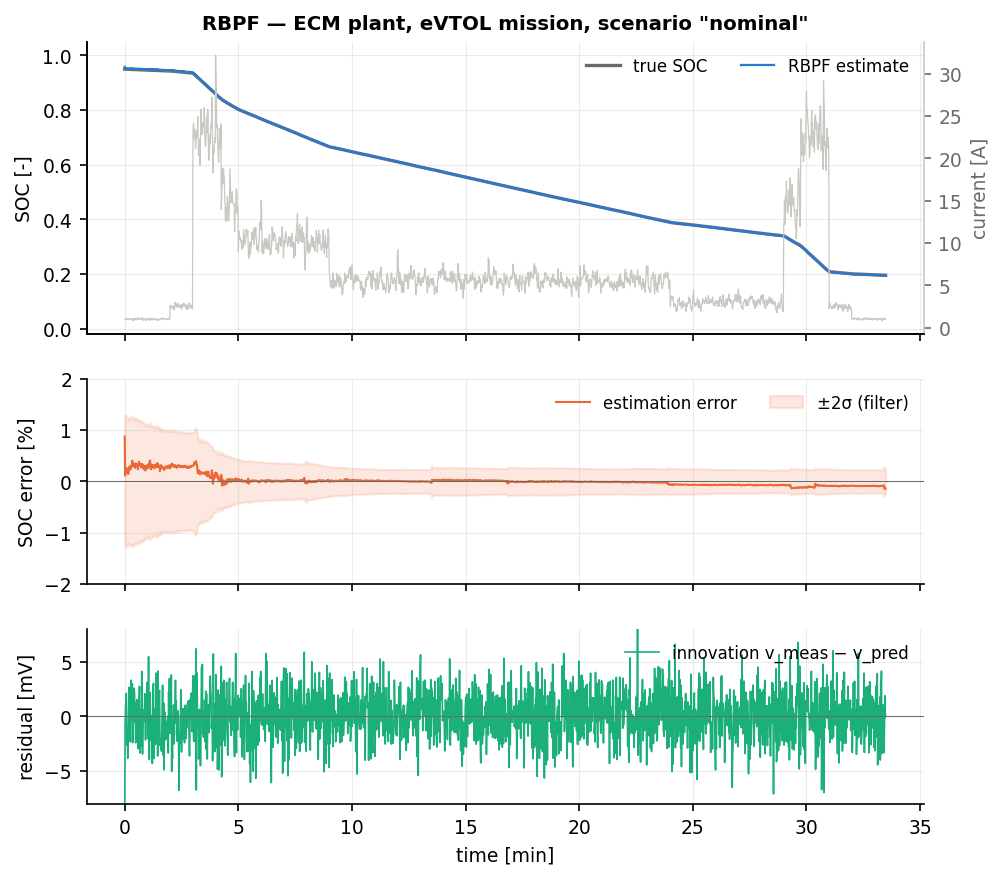
\includegraphics[width=\textwidth]{figures/cell_RBPF_nominal.png}
\caption{RBPF on the nominal eVTOL mission: true and estimated SOC (top), estimation error with the
$\pm2\sigma$ band from the Gaussian-mixture covariance \eqref{eq:rb-cov} (middle), voltage residual
(bottom).}
\end{figure}
\begin{figure}[H]\centering
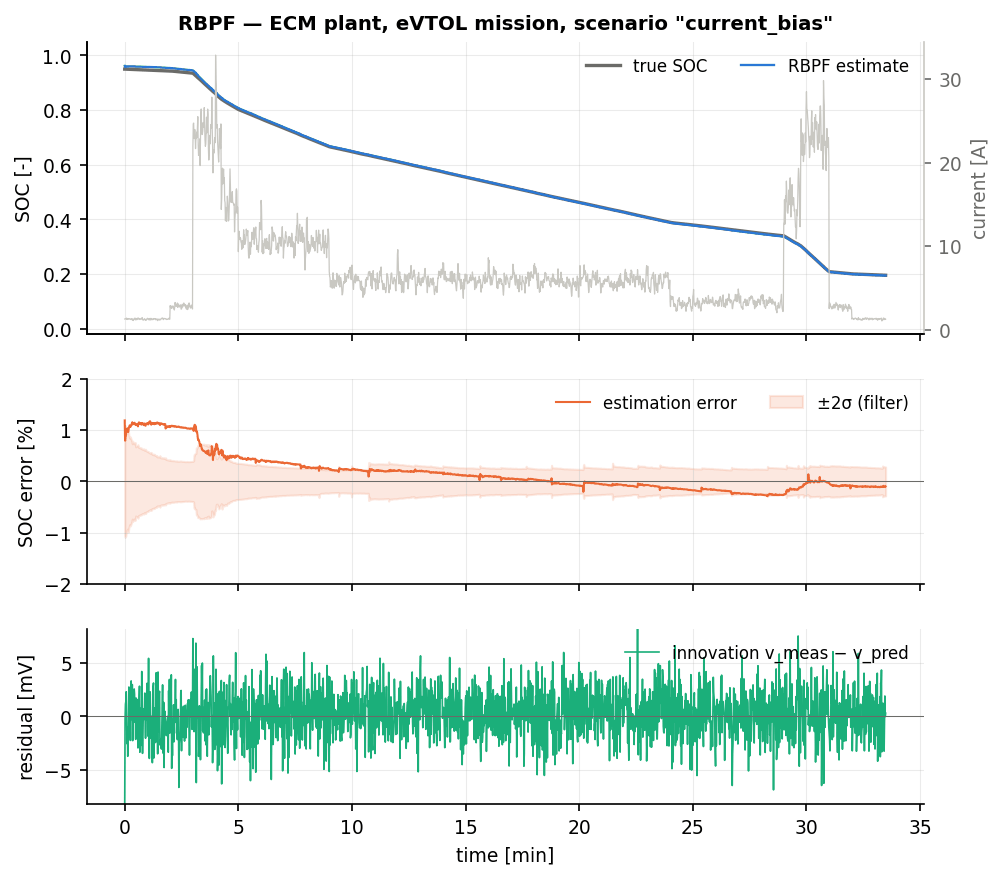
\includegraphics[width=\textwidth]{figures/cell_RBPF_current_bias.png}
\caption{RBPF on \code{current\_bias} (\SI{0.25}{\ampere} offset, \SI{2}{\percent} gain error):
\SI{0.12}{\percent} steady-state SOC error, five times better than the EKF and the best result of
any method in this family on this scenario.}
\end{figure}
\begin{figure}[H]\centering
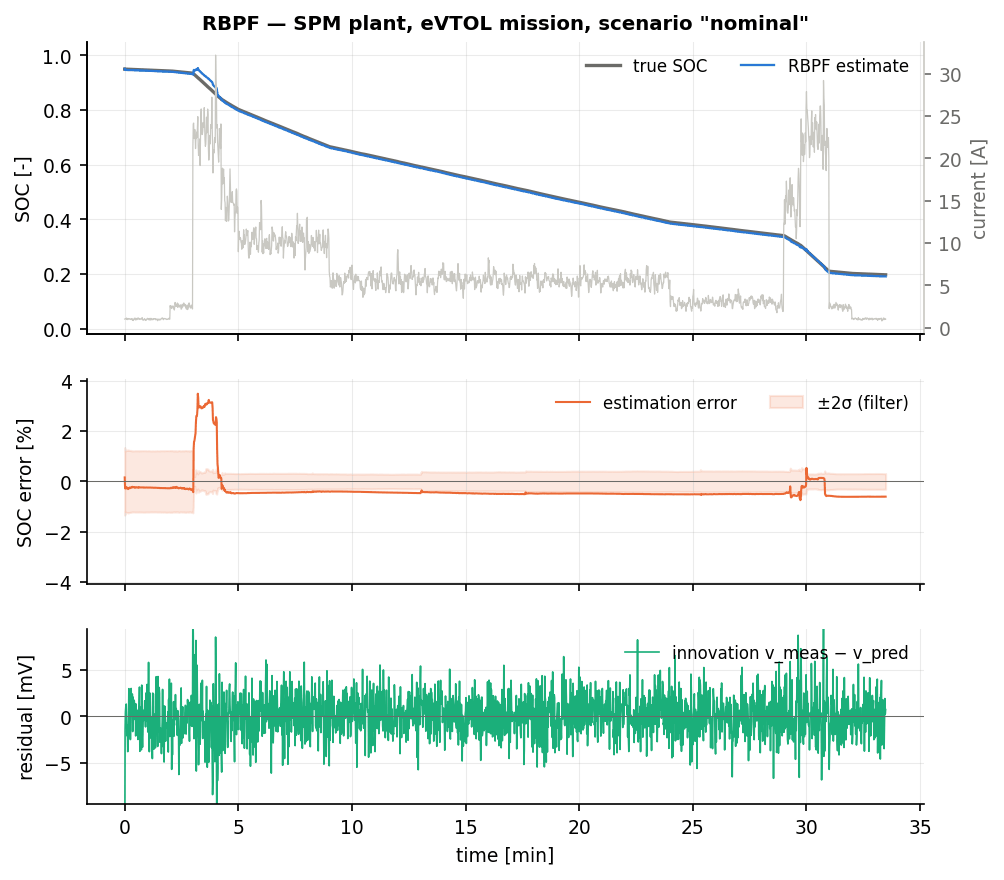
\includegraphics[width=\textwidth]{figures/cellspm_RBPF_nominal.png}
\caption{RBPF on the electrochemical (SPM) plant, nominal mission.  The conditional Kalman filters
absorb the structured residual optimally \emph{for the assumed model}, which is both why the
estimate stays smooth and why the SOC error is larger than for the full-state particle filters.}
\end{figure}

\paragraph{ECM plant --- accuracy.}  On \code{nominal} the RBPF reaches
$\mathrm{RMSE} = \SI{0.14}{\percent}$, $\mathrm{RMSE}_{\mathrm{ss}} = \SI{0.06}{\percent}$ and a
voltage-residual RMSE of \SI{0.80}{\milli\volt}: level with the EKF (\SI{0.05}{\percent}) and the
UKF (\SI{0.04}{\percent}) on a plant whose model is exact, second only to the Gaussian-sum filter
(\SI{0.05}{\percent}) within this family, and a factor \num{2.7} better than the 500-particle
bootstrap filter at half its cost.  That factor is the Rao--Blackwell reduction
\eqref{eq:rb-total-variance} made visible: same algorithm, same roughening, two sampled dimensions
instead of four.

The advantage widens where model error, not measurement noise, dominates:
\begin{itemize}[leftmargin=2em]
  \item \code{current\_bias} (\SI{0.25}{\ampere} offset, \SI{2}{\percent} gain error):
        $\mathrm{RMSE}_{\mathrm{ss}} = \SI{0.12}{\percent}$, against \SI{0.87}{\percent} for
        \estname{PF-Bootstrap}, \SI{0.61}{\percent} for the EKF and \SI{0.57}{\percent} for the UKF
        --- a factor of five to seven, and the best result of any estimator in this family.  With
        $v_1,v_2$ handled exactly, the persistent voltage residual caused by the current bias is
        attributed to SOC rather than being smeared across sampled RC voltages.
  \item \code{combined}: \SI{2.05}{\percent}, the best of the entire family and a factor \num{6.1}
        better than the EKF's \SI{12.44}{\percent} (which never converges).
  \item \code{aged\_cell} \SI{2.25}{\percent} and \code{param\_mismatch} \SI{1.53}{\percent}, the
        best of the five particle filters on both.
  \item \code{cold} \SI{0.18}{\percent} and \code{hot} \SI{0.07}{\percent}: the temperature
        scheduling acts almost entirely on $\mA_l$ and $\bm b_l$, which the RBPF treats
        analytically.
  \item \code{preisach} \SI{0.40}{\percent} --- by far the best of the particle filters (the
        full-state ones are at \SIrange{1.00}{1.08}{\percent}), because the hysteresis state is one
        of the two that are \emph{sampled}, so the corrected Preisach bias is met by an explicit
        multi-hypothesis search rather than by a jitter.
\end{itemize}

\paragraph{ECM plant --- the weakness: a large initial error.}
With a \SI{35}{\percent} initial SOC error the RBPF converges only after \SI{309}{\second}
(steady-state \SI{0.35}{\percent}, whole-run RMSE \SI{2.66}{\percent}), and \code{outliers} is its
other soft spot (\SI{0.68}{\percent}, the worst of the five particle filters, with convergence at
\SI{110}{\second}).  Both have the same cause, and it is a property of the method rather than a
defect of the implementation.  At $k=0$ the conditional Kalman filter of every particle sees a
\SI{250}{\milli\volt} residual and a prior in which $\sigma_{v_2} = \SI{5}{\milli\volt}$ against a
measurement noise of \SI{2.1}{\milli\volt}; conditioned on a \emph{fixed} SOC, the only way to
explain that residual is $v_1 + v_2$, so the Kalman gain $\mK^i \approx \num{0.74}$ pushes $v_2$ to
about \SI{-185}{\milli\volt}.  Every particle then explains the data equally well, the marginalised
likelihoods \eqref{eq:rb-marglik} become nearly equal, and the SOC weights carry almost no
information.  Only as the physically decaying RC states relax on their $\tau_2 = \SI{120}{\second}$
time scale does the residual reappear and the SOC selection resume.  A joint Gaussian update --- what
the EKF does --- does not have this problem, because there the SOC prior variance dominates the
innovation covariance and the correction goes almost entirely into SOC.  A \SI{50}{\milli\volt}
outlier is absorbed the same way and takes a few RC time constants to leave.  This is the RBPF's
structural trade: conditioning on $\vx_n$ is what buys the variance reduction, and it is also what
prevents an SOC-dominated interpretation of a single large residual.

\paragraph{SPM plant.}  Against the electrochemical plant the RBPF gives
$\mathrm{RMSE}_{\mathrm{ss}} = \SI{0.76}{\percent}$ on \code{nominal}, a factor \num{4.9} better
than the EKF's \SI{3.73}{\percent} and \num{5.2} better than the UKF's \SI{3.96}{\percent}.  It is,
however, the \emph{weakest} of the five particle filters there (auxiliary \SI{0.62}{\percent},
regularised \SI{0.64}{\percent}, bootstrap \SI{0.73}{\percent}), and the gap widens on the harder
SPM rows: \code{current\_bias} \SI{2.37}{\percent} against \SI{0.89}{\percent} for
\estname{PF-Auxiliary}, \code{noise\_step} \SI{2.76}{\percent} against \SI{1.01}{\percent},
\code{hot} \SI{1.88}{\percent} against \SI{0.59}{\percent}, and SPM \code{init\_error} never reaches
the \SI{2}{\percent} band at all (\SI{4.71}{\percent}).

The reason is the same mechanism as the ECM initial-error weakness, now driven continuously instead
of once.  The full-state particle filters keep $v_1,v_2$ as \emph{sampled} coordinates that the
roughening jitter continuously re-randomises, so the cloud is free to place the structured
\SI{4}{\milli\volt} residual wherever the likelihood prefers --- in practice on the slow RC state
and in the voltage residual.  The RBPF instead computes, for each sampled $(\soc,h)$, the
\emph{optimal} $(v_1,v_2)$ posterior \emph{under the assumed 2-RC model}.  When that model is wrong
the optimum is wrong in a specific, correlated way: the conditional Kalman filter drives $v_1,v_2$
to whatever reproduces the measured voltage given the particle's SOC, which restores exactly the
linearised $(\soc, v_2)$ ambiguity that marginalisation was supposed to remove, and the marginalised
likelihoods \eqref{eq:rb-marglik} become nearly equal across the cloud again.  Rao--Blackwellisation
is only free when the conditional model is correct; against structured model error it converts a
Monte-Carlo variance reduction into a modelling bias.  The honest summary is that the RBPF is the
best choice on the matched plant and a mid-field choice on the mismatched one --- still five times
better than the EKF, but no longer the leader.

\section{Summary}
The marginalised particle filter samples only what must be sampled.  For the 2-RC cell model the
partition is exact: SOC and hysteresis are sampled, the two RC voltages are integrated out by a
$2\times2$ Kalman filter attached to every particle, and the importance weights use the analytically
marginalised likelihood.  The law of total variance guarantees that this cannot be worse than
sampling all four states \emph{of the same model}, and on the ECM plant it shows: \SI{0.06}{\percent}
on \code{nominal} (level with the EKF, \num{2.7} times better than a 500-particle bootstrap filter
at half the cost), the best current-bias result in the library (\SI{0.12}{\percent} against the
EKF's \SI{0.61}{\percent}), the best \code{combined} (\SI{2.05}{\percent} against \SI{12.44}{\percent})
and the best particle-filter \code{preisach}.  Its two weaknesses share one cause --- conditioning on
a fixed sampled SOC lets the RC branches absorb any large or persistent residual: recovery from a
\SI{35}{\percent} initialisation error takes \SI{309}{\second}, and on the electrochemical plant,
where the residual is structural and permanent, it falls behind the full-state particle filters
(\SI{0.76}{\percent} against \SI{0.62}{\percent}) while still beating the EKF fivefold.  Use it as
the reference particle filter for a conditionally linear model you trust; use a full-state filter,
or a Kalman filter to bootstrap it, when you do not.
